\documentclass{sig-alternate}
  \pdfpagewidth=8.5truein
  \pdfpageheight=11truein

\usepackage{listings}
\usepackage{graphicx}
\usepackage[pdftex,hypertexnames=false,bookmarks=false,linkbordercolor={.9 .9 1}]{hyperref} 

\newcommand{\codefamily}{\sffamily}
\newcommand{\csharp}{C\#}
\newcommand{\code}[1]{\lstinline{#1}}

\title{Embedded Contract Languages}
\numberofauthors{3} %  in this sample file, there are a *total*

\author{
% You can go ahead and credit any number of authors here,
% e.g. one 'row of three' or two rows (consisting of one row of three
% and a second row of one, two or three).
%
% The command \alignauthor (no curly braces needed) should
% precede each author name, affiliation/snail-mail address and
% e-mail address. Additionally, tag each line of
% affiliation/address with \affaddr, and tag the
% e-mail address with \email.
%
% 1st. author
\alignauthor Manuel F\"ahndrich\\
       \affaddr{Microsoft Research}\\
       \email{maf@microsoft.com}
% 2nd. author
\alignauthor Michael Barnett\\
       \affaddr{Microsoft Research}\\
       \email{mbarnett@microsoft.com}
% 3rd. author
\alignauthor Francesco Logozzo\\
       \affaddr{Microsoft Research}\\
       \email{logozzo@microsoft.com}
}
%\author{Manuel F\"ahndrich, Michael Barnett, and Francesco Logozzo}

\begin{document}
% --- Author Metadata here ---
\conferenceinfo{SAC'10}{March 22-26, 2010, Sierre, Switzerland.}
\CopyrightYear{2010} % Allows default copyright year (2002) to be over-ridden - IF NEED BE.
\crdata{978-1-60558-638-0/10/03}  % Allows default copyright data (X-XXXXX-XX-X/XX/XX) to be over-ridden.
% --- End of Author Metadata ---

\maketitle
\begin{abstract}
Specifying application interfaces (APIs) with information that goes
beyond method argument and return types is a long-standing quest of
programming language researchers and practitioners. The number of
type system extensions or specification languages is a testament to
that. Unfortunately, the number of such systems is also roughly equal to
the number of tools that consume them. In other words, every tool
comes with its own specification language.

In this paper we argue that for modern object-oriented languages,
using an \emph{embedding} of contracts as code is a better
approach. We exemplify our embedding of Code Contracts on the
Microsoft managed execution platform (.NET) using the \csharp{}
programming language. The embedding works as well in Visual Basic.  We
discuss the numerous advantages of our approach and the technical
challenges, as well as the status of tools that consume the embedded
contracts.
\end{abstract}
\vspace*{-3mm}
% A category with the (minimum) three required fields
\category{D.2.4}{Software Engineering}{Software/Program
  Verification}[Programming by contract]
\category{D.2.1}{Software Engineering}{Requirements/Specifications}[Methodologies, Tools]
\category{F.3.1}{Logics and Meanings of Programs}{Specifying and
  Verifying and Reasoning about Programs}[Assertions, Invariants, Pre-
  and post-conditions, Specification techniques]
\vspace*{-7mm}
\terms{Design, Languages, Reliability, Verification}
\vspace*{-3mm}
\keywords{C\#, .NET, CodeContracts}
\vspace*{-3mm}

\lstset{language={[Sharp]C},mathescape=false,flexiblecolumns=true,morekeywords={alloc,delay,delete,expose,let,unsatisfiable,receive,rep,contract,message,state,one},basicstyle=\codefamily\small,literate={->}{{$\rightarrow$}}{2}{<<}{{$\langle$}}{2}{>>}{{$\rangle$}}{2}{!}{{\textbf{!}}}{2},frame=lines,moredelim=[is][\itshape]{@}{@},captionpos=b,numberstyle=\tiny,stepnumber=1,numbersep=2pt}

\section{Specifications and Contracts}
\noindent
Writing specifications for programs and verifying these specifications
against the actual code (either dynamically or statically) has a long
tradition in the research community. Specifications and their
corresponding checkers take on a multitude of forms, from simple
extensions to type
systems~\cite{Deline04typestatesfor,nonnull,pluggable}, dependent
types~\cite{DML}, monitors~\cite{Ball04slamand,OpalDas06}, to full
fledged logical specification and
verification~\cite{eiffel,Leavens-Baker-Ruby06,SpecSharp,vcc,Dana,adaspark}.

\noindent
One of the recurring issues with specification languages is that they
are either very specialized and limit the expressiveness of what
properties can be expressed (often towards the goal of static
checking), or they are general specification languages either with
their own specialized programming
language~\cite{eiffel,SpecSharp,vcc,Dana,adaspark}, or augmenting an
existing language via structured
comments~\cite{Leavens-Baker-Ruby06}. In either case, these approaches
require entire compiler infrastructures to support tools consuming the
specifications. Specialized languages are difficult to get into
general usage, as the compilers and support tools are usually not on
par with commercial product quality. Often such infrastructures need
to track the evolution of some original language (Spec\# vs. C\# and
JML vs. Java), which means they either don't support the same
language, or lag several years behind the features of the main
language.  Comment- and annotation-based approaches have additional
problems that we discuss in the next section.

To avoid all these issues, we propose a novel approach based on
embedding contract specifications in a programming language without
any change to the programming language and taking full advantage of
the existing language, compiler, and its supporting IDE and tools.

\begin{figure}[bt]
\begin{center}
\begin{lstlisting}
string Compute(string str,int index,Collection c,out int len)
{
  Contract.Requires(str == null ||
                    0 <= index && index < str.Length);
  Contract.Ensures(str == null ||
                   !String.IsNullOrEmpty(Contract.Result())
                   && c.Count > Contract.OldValue(c.Count));
  Contract.Ensures(Contract.ValueAtReturn(out len) >= 0 );
  Contract.Ensures(str == null || Contract.ForAll(
                    0, Contract.ValueAtReturn(out len),
                    i => Contract.Result()[i] == s[i]) );
}
\end{lstlisting}
\end{center}
\vspace*{-5mm}
\caption{Example of embedded contracts}
\label{fig:example}
\vspace*{-3mm}
\end{figure}

\section{Embedded Contracts}
\label{sec:embeddings}
\noindent
The idea of embedding contracts in an existing programming
language is to
\begin{enumerate}
\item express specification conditions as expression in the
programming language itself, to
\item leverage the existing language
compiler to perform name and overloading resolution, type checking,
and code generation, and to
\item extract contract conditions from the compiled target code for
  use in contract related tools.
\end{enumerate}

\noindent
Figure~\ref{fig:example} shows our embedding of contracts for
\csharp{}. The method \lstinline{Compute} specifies a precondition
using a boolean expression that is the argument to the
\lstinline{Contract.Requires} method. It also specifies several
postconditions using boolean expressions as the argument to the
\lstinline{Contract.Ensures} method.

In this embedding, contract specifications appear as method calls at
the beginning of methods, where the specification conditions are
simply the boolean expressions appearing as arguments to these
methods. In .NET we are using static void methods defined in a static class
called \lstinline{Contract}. Other approaches are possible using
global objects and methods.

Using an embedded approach for writing specifications provides
numerous benefits to the programmer:
\begin{itemize}
\item  The language of conditions is just the language of 
expressions in the programming language used.
\item The existing editor and IDE can not only be used to author the
  contracts, the IDE actually supports writing proper contract
  expressions by providing highlighting, completion, intellisense, and
  early feedback on erroneous expressions (due to the fact that the
  existing language will background check the expressions as normal
  code).
\item Refactoring tools work properly on contracts as well, e.g.,
  renaming a parameter will rename any parameter use inside
  specifications as well. Contrast this to having specifications in
  attributes or special comments.
\end{itemize}

\noindent Thus, programmers don't have to learn a new language, a new compiler,
or a new IDE, and the authoring of contracts feels like writing code.


Embedding is also beneficial to writers of tools such as dynamic and
static contract checkers:
\begin{itemize}
  \item Since the specifications are compiled by the existing
    compiler, the tool writer has no need to duplicate the full
    compiler infrastructure, such as the parser, type
    checker, name and overloading resolution, etc., or extend the IDE
    to recognize specifications in non-standard positions, such as
    attribute strings or comments.

  \item Extracting the specifications from the compiled target code as
    opposed to the source code allows the tool writer to deal with a
    smaller and usually better specified language than the original
    source language. In our example, consider the difference in
    complexity between the full \csharp{} language and the relative
    simplicity of the target MSIL intermediate language of .NET.
    
  \item The semantics of the expressions appearing in the
    specifications are unambigous. Consider operator overloading and
    other special language constructs. Working at the source level of
    expressions would require tool writers to duplicate the knowledge
    of how such operators are translated. Working in the target
    language obviates this need.

  \item The tool writer can typically reuse existing well tested
    infrastructure to manipulate/analyze the target code, such as .NET
    binary reader/writers, or similarly Java byte code
    infrastructures.
\end{itemize}

\noindent Embedding a contract language also presents some challenges over
alternative approaches. We examine these challenges in the next sections and
provide solutions for them.

\begin{figure}[tb!]
\begin{center}
\begin{lstlisting}
[ContractClass(typeof(IContracts))]
interface I {
  int Foo(string s);
}

[ContractClassFor(typeof(I))]
class IContracts : I {
  int Foo(string s) {
    Contract.Requires( s != null );
    Contract.Requires( s.Length > 5);
    Contract.Ensures( Contract.Result() > 0 );

    return default(int); // dummy body
  }
}
\end{lstlisting}
\end{center}
\vspace*{-5mm}
\caption{Contracts on interface methods}
\label{fig:interfacecontracts}
\vspace*{-3mm}
\end{figure}

\subsection{Common Specification Encodings}
\noindent
While reusing the existing language for expressions appearing in
specifications is great, it also poses a problem in that specification
languages usually require a few extra constructs not typically among
the expressions of standard programming languages.

\subsubsection{Method Result Expression} 
\noindent
Postconditions often need to refer to the method result
value. Languages typically don't have an expression form for this
result value. To work around this issue, we use a dummy nullary method
whose result stands for the result value of the method:
\begin{lstlisting}
  static T Result<T>();
\end{lstlisting}
The type parameter \code{T} stands for the method return type. Some
languages can infer this type, but often programmers will need to
specify it.
An example use appears in Figure~\ref{fig:example}, where the
postcondition ensures that the result string is neither null, nor empty.

\subsubsection{Prestate Values}
\noindent
It is convenient to mention the \emph{old value} of an expression in a
postcondition, meaning the value of the expression on entry to the
method. This is typically used to related the pre and the post state,
e.g., to express that a count was incremented, an element was added,
etc.

Again, standard programming languages don't have syntax for such a
construct and we make use of a unary dummy function with the following signature:
\begin{lstlisting}
  static T OldValue<T>(T oldExpression);
\end{lstlisting}

\subsubsection{Contracts on Interfaces}
\noindent
Writing contracts on interface declarations is very desirable, but not
straightforward. Since we use code in method bodies to express contract
conditions and interface methods don't typically allow writing method
bodies, we have to find a way to write the contracts separately from
the interface declaration and link the two. 

To annotate an interface \lstinline{I} with contracts, we use a \emph{buddy}
contract class, typically named \lstinline{IContracts} that implements
the interface and for each method contains the contracts and a dummy
body (Figure~\ref{fig:interfacecontracts}).
The interface type and its contract class are linked in our \csharp{}
embedding using attributes. An alternative mechanism could use naming conventions.

\subsubsection{Quantifiers}
\noindent
Specifications often require universal or existential quantifiers
which are not typically available in mainstream programming
languages. Fortunately, modern languages now provide support for
closures, making it possible to express quantifiers as helper methods
in ordinary expressions. Figure~\ref{fig:example} contains a
postcondition using a universal quantification over the range
$0..\mathsf{len}$. The bound variable and universally quantified
boolean expression is represented in \csharp{} as a lambda expression 
\begin{lstlisting}
 i => <expression over i>
\end{lstlisting}
where \lstinline{i} is a bound variable and
 \lstinline{<expression over i>}
is the lambda body.

In our \csharp{} embedding, we provide several overloads of
\lstinline{ForAll} and \lstinline{Exists} that work over integer
ranges and collections. In the example, we use the following:
\begin{lstlisting}
delegate bool Predicate<T>(T value);
bool ForAll(int lb, int ub, Predicate<int> condition);
\end{lstlisting}
Unbounded quantification can be
expressed as well, but poses obvious problems for runtime checking.

\subsubsection{Object Invariants}
\noindent
Object invariants are conditions on object state that should hold on
all public method boundaries. Such invariants need to be specified at
the type level, but languages again don't provide a way to associate
code directly with types. Instead, we embed object invariants by
defining additional instance methods on types and marking them as object
invariants as shown below in our \csharp{} embedding:
\begin{lstlisting}
[ObjectInvariantMethod]
void ObjectInvariant() {
  Contract.Invariant( this.field >= 0 );
}
\end{lstlisting}
These invariant methods take no parameters and return no result. The
body consists of a sequence of \lstinline{Contract.Invariant} method
calls specifying the invariant conditions.

\subsubsection{Language Workarounds}
\noindent
Programming language rules may get in the way of certain embedding
usages, namely due to the fact that postconditions appear at the
beginning of the method rather than where they are evaluated. E.g., 
\csharp{} supports \emph{out-parameters} which are parameters passed by
reference that need not be initialized on entry, but the method is
guaranteed to assign them. \csharp{} enforces the rule that such
parameters are not read before being assigned. A postcondition
referencing an out-parameter will be flagged by
the compiler as a use-before-assignment. To work around this and
related issues in constructors, we provide a helper method whose
meaning is that the location is read in the post state.
\begin{lstlisting}
  static T ValueAtReturn<T>(out T location);
\end{lstlisting}
Figure~\ref{fig:example} contains a postcondition stating that the
value upon return of the out-parameter \lstinline{len} is non-negative.

\subsection{Other Specification Encodings}
\noindent
There are a number of specification language features that we have not
yet attempted to support in our encodings and tools. We list them here
and provide ideas for how to encode them. 

\textit{Model Fields} are data members or properties of data
structures that are typically only referred to from specifications
rather than real code. They can be expressed as ordinary 
virtual properties, tagged with special attributes. Concrete
implementations then act as the representation formuala.

\textit{Modifies Clauses} describe the set of locations potentially
modified by a method. A set of dummy methods, similar to
\lstinline{ValueAtReturn}, can be used to express classes of such
locations. 

\textit{Data Groups}~\cite{datagroups} are typically used to abstract
over sets of locations, including recursively defined sets in order to
express which parts of the machine state are (un)modified. We
envision that such groups can be encoded with extra attributes.

Finally, specification languages often use \textit{Model Types}, i.e.,
mathematical structures such as sets and sequences to express
properties of implementation data structures. Spec\# supports such
model types as actual .NET implementations of functional data
structures. The same approach can be used in an embedded setting.


\section{Contract Extraction}
\label{sec:extraction}
\noindent
Contract extraction consists of separating the code generated for
contract conditions (preconditions and postconditions) inside a method
from the code making up the body of the method.

For ordinary methods, code extraction is relatively simple. It
consists of finding the last use of a contract method
(\lstinline{Requires} or \lstinline{Ensures}) and then splitting up all code
from the beginning of the method to that point into individual pre- and
postconditions. This process must ensure certain well-formedness
conditions in order to guarantee that the contracts and code can be
properly separated:
\begin{itemize}
\item Each individual pre- and postcondition must post-do\-minate the
  entry point of the method. This guarantees that the contracts
  actually appear at method entry and are not control-flow dependent.

\item Local variables initialized inside contracts must not be used inside
  the method body. This guarantees that contracts can be separated
  from the method body without having to perform detailed dependency
  analysis and to duplicate local initializations.

\item No references to contract helper methods should appear in the
  main method body. This guarantees that the special meaning of
  contract helper methods only needs to be recognized as part of the
  contracts themselves.

\item Preconditions can only mention types and members that are
  visible to all callers of the method. This guarantees that callers
  can understand the contract they are held to and avoids having
  meaningless preconditions, e.g., on private object state.

\item Postconditions of virtual methods can only mention types and members that are
  visible to all potential implementers of the method. This guarantees
  that overrides and implementations of the method 
  can understand the postcondition they are held to.

\item Contract helper methods such as \lstinline{OldValue},
  \lstinline{Result}, and \lstinline{ValueAtReturn} should only be
  referenced from within postconditions. Furthermore, the type
  instantiation of the \code{Result} method should agree with the
  method return type.

\item Contract inheritance of preconditions should be checked to
  guarantee that methods don't strengthen preconditions. A simple way to
  enforce this without needing to determine arbitary logical
  implications is to simply disallow overriding methods from declaring
  their own preconditions and further guaranteeing that methods only
  have one base method (base class or interface) from which they
  inherit contracts.

\item Any methods called from within contract expressions should be
  pure methods (or referentially transparent) to avoid issues of
  contract semantics and changing the behavior of the program
  depending on whether contract assertions are evaluated at runtime or
  not.  We advocate
  requiring a purity annotation on methods called from contracts such
  as \code{[Pure]} to 1) document the intention of the method's purity
  and thus capturing it in the code, and 2) enable a separate analysis
  to discharge the purity obligation of such annotated methods.

  Additionally, methods used in contracts should be well-founded to
  avoid ill-defined specifications. 
  Checking methods for purity and well-foundedness is non-trivial and
  beyond the scope of discussion for this paper.
\end{itemize}
Contracts need to be cleanly separated from ordinary code in order to
enable manipulating the code for various runtime checking
scenarios, such as removing all contract code, inheriting contract
code to overridden methods, and inserting contract checking code at
call-sites of methods.

\subsection{Challenges}
\noindent
The basic extraction of contracts from methods is fairly simple as
described above. Challenges arise when the code generated by the
compiler is substantially more complicated than the source due to
expansion of certain language features. 

\subsubsection{Constructors}
\noindent
Extraction from constructor methods is more complicated than for
ordinary methods due to two issues: 1) base or delegated constructor calls, and 2)
field initialization. Depending on the language, field initialization
may appear before or after the base/delegated constructor call (e.g.,
\csharp{} puts field initialization before, Visual Basic puts them
after). This makes recognizing the beginning of contracts more
difficult, as they will appear after all the field initializations and
base constructor call.

Another complication with constructors is that even though
preconditions physically appear after the base/deferred constructor call,
logically, the preconditions must be evaluated prior to the base/deferred
constructor call. Prior to that call, the object being constructed is
not yet accessible (fields may be written but not read and the object may
not escape). As a result, preconditions in constructors must be
checked to contain no references to the object under construction.

\subsubsection{Closures}
\noindent
Most modern object oriented languages now support closures (or
anonymous delegates) in one form or another. If the underlying target
language does not support this feature directly, the compiler will
emit helper types and methods to implement the feature, complicating
the contract extraction. E.g., if a closure is used inside a contract,
then the method code will contain closure object initialization
code. Such code needs to be part of the contract code, but may also
need to be part of the ordinary method body, since compilers will try
to share the closure object between the two sections. As a result,
such closure construction code has to be specially recognized and
considered to be part of both the contract section and the normal
method body.

\subsubsection{Iterator Methods}
\noindent
Languages like \csharp{} and Visual Basic support iterator methods,
i.e., methods producing an enumeration of values that can be written
in the form of a coroutine using \lstinline{yield} statements to yield
individual values.

Compilers turn such iterator methods into iterator closure classes that
implement enumeration interfaces. The code transformations are quite
substantial, causing the embedded contracts to end up inside a
different compiler generated method
body for advancing to the next element of the iteration. To extract
contracts properly from iterators, the extraction process must
essentially recognize such iterators and partially decompile them.

\section{Modularity}
\noindent
Before discussing tools built on top of embedded contracts, we need to
discuss the issue of how to handle separate compilation and contracts
of third-party components.

We view every component (be it a .NET assembly, or a Java class file,
or other packaging granularity) as having a set of declared
contracts. Tools working on a component $A$ referencing a component
$B$, typically need to obtain the contracts of component $B$,
independently of whether $B$ is instrumented with runtime checks or
not. We therefore introduce the notion of a \emph{Contract Reference
 Component} (CRC), such that for every component $A$ there is a CRC
called $A.Contracts$ containing only contracts, no method bodies.
One way to think about a CRC is as a rich header file giving detailed
contract information beyond the typical type signatures.

Note that a CRC is a persisted form of the contracts in the
source. The format of this persisted form is already given by whatever
compiler target language we are employing, e.g., .NET or JVM. This
again simplifies the contract story, as contracts in component
reference assemblies have the same fixed semantics we have already
assigned to the target language.

CRCs simplify dealing with multiple components and also permit
writing contracts for components separately if the component does not
originally contain contracts. It simplifies the description of
tools acting on components. For the remainder of the paper, we assume
that we can compile a component in such a way that it contains no
contracts, to yield the uninstrumented pristine compiled component $A$. For
\csharp{} and Visual Basic, we use the \code{Conditional("Contracts")} compilation
attribute on all the \code{Contract} methods which causes the
compilers to omit any calls to these methods when the compilation is
performed without defining the symbol "Contracts".

Note that this approach permits authoring contracts on components,
while guaranteeing that the non-contract code can easily be compiled
into pristine form (i.e., containing just the non-contract code) with
the standard compilers without any other tool in the process. This
ability is important for adoption by product teams if they don't trust
other tools to modify their code before shipping.

We can thus view the standard language compilers as our first tool in
the contract toolbox. The next tools we need is the CRC generator,
generating a contract reference component.

\section{Tools}
\noindent

\subsection{CRC Generation}
\label{sec:ccrefgen}
\noindent
Generating a contract reference component is simple: Compile the
original code with contracts and then rewrite this component $A$ to strip the method bodies and
persist only the contracts as $A.Contracts$. 

It is useful to perform an extra step in CRC generation, namely to
persist the original source string of any contract conditions as part
of the method calls to \code{Contract.Requires},
\code{Contract.Ensures}, and \code{Contract.Invariant}. Effectively,
what this step does is it turns any code of the form
\begin{lstlisting}
  Contract.Requires( expr );
\end{lstlisting}
into
\begin{lstlisting}
  Contract.Requires( expr, "expr"); 
\end{lstlisting}
and similarly for \code{Ensures} and \code{Invariant}.

In order to perform this rewriting, we assume (or emit) binary forms
of the contract methods that take an additional string argument after
the boolean condition. Persisting the original source of the condition
in this manner permits downstream tools to emit better error messages
that can display the original condition that fails without the need to
decompile a low-level target language into readable source.

The source extraction is done by using source debugging file information on
the compiled target to help locate the correct source file and text
extent.

\subsection{Runtime Contract Checking}
\noindent
A principal use of contracts is to instrument contract checks as
runtime assertions into the target code. Runtime checking increases
test effectiveness as the extra assertions provide expected outcomes
(oracles) and provide more ways to fail the code under test. Runtime
contract checking is particularly effective in conjunction with
automated testing, such as fuzzing~\cite{DBLP:journals/tse/Korel90,DBLP:conf/popl/Godefroid07}, and automated white-box testing~\cite{DBLP:journals/cacm/King76,DBLP:conf/kbse/GuptaMS00,DBLP:conf/tap/TillmannH08}.

Runtime checking can be instrumented on a component basis (or finer grained
if desired). To instrument a component $A$, we need the pristine form
of $A$, along with its CRC $A.Contracts$, as well as any CRCs
$B.Contracts$, for any component $B$ referenced by $A$.

Instrumentation can support different levels by including/omitting
certain kinds of checks. Here we describe how our implementation
instruments all contracts.

We view instrumentation as a rewriting of component $A$ into $A'$,
where $A'$ contains runtime assertions for contracts, but is otherwise
identical to $A$. In particular, the actual name of the instrumented
component does not change, but we use the primed version to simplify
the explanation. 

Rewriting proceeds on a per class basis, in an order where base
classes (in the same component) are visited prior to derived classes. 

\subsubsection{Runtime Failure Behavior}
\noindent
Runtime failure of contracts should be customizable, as different
scenarios require different behaviors. E.g., standard interactive
debugging scenarios may want contract failure to pop-up a dialog box
with the option to enter the debugger. Automated testing environments
usually need failure in the form of a thrown exception, while
deploying instrumented code scenarios may require the component to
abort or to log failures in a file or over the network.

We therefore don't advocate any particular failure behavior, but leave
that up to the instrumentation tool and the user's choice. All we
assume is that the runtime failure operation has access to the source
string representing the original contract condition in order to
provide a meaningful level of detail about the failed contract.

\subsubsection{Invariants}
\noindent
The various object invariant methods declared on a type are
consolidated into a new method with a fixed name that does not clash
with user defined method names, e.g., \code{\$invariant\$}. This
\code{\$invariant\$} method is a protected instance method containing
all \code{Contract.Invariant} checks of all contract invariant
methods. In addition, if the base class contains a \code{\$invariant\$}
method, then this means that the base class is instrumented and we can
chain the invariant checking by calling this base method.

At the end of selected methods (e.g., all public methods), calls to
this generated \code{$invariant$} method can be inserted to validate
the object invariant.

\subsubsection{Preconditions}
\noindent
If contracts are well-formed (Section~\ref{sec:extraction}), a method only has
one source of preconditions, either the method itself, or if it
overrides/implements a base method, the base method's preconditions.

Instrumenting a precondition declared on the method itself is trivial,
as the precondition can simply be copied in its existing form to the
beginning of the method. 

When inheriting a precondition, complications arise. The base class
could be generic, and thus the base contract must be instantiated with
the same instantiation used by the base type declaration. In target
languages where generic code is compiled away (JVM), such
instantiation is trivial, as it does not require changing the
inherited code for the precondition. In target languages where
generics are explicit however, such as .NET, the inherited code has to
be properly instantiated before being emitted, or the runtime will
reject the code.

\subsubsection{Postconditions}
\noindent
Runtime checking of postconditions is more complicated due to the
presence of the special \code{Contract} methods such as \code{Result},
\code{OldValue}, and \code{ValueAtReturn}. The simplest of the three
is \code{ValueAtReturn}, which can simply be replaced by a dereference
operation of the by-ref location. 

\textbf{Return values:} To handle \code{Result}, we first replace all return points in the
method with assignments to a new \code{$result$} local and a branch to
a common method exit point where the post conditions will be checked. 
Any calls to \code{Contract.Result} in the postcondition code can then
be replaced with uses of the \code{$result$} local variable.

\textbf{Old-expressions:} Dealing with \code{OldValue} requires evaluating the expression
serving as the argument to \code{OldValue} in the prestate of the
method and storing the result away in a fresh local variable. Each
occurrence of a call to \code{OldValue} in the postconditions is then
replaced with the corresponding local variable. 

Due to shortcut evaluation constructs such as \code{||}, \code{&&},
and conditional expressions present in most languages, \code{OldValue}
expressions may not and should not be evaluated unconditionally. E.g.,
consider the postcondition:
\begin{lstlisting}
int M(C c) 
{
  Contract.Ensures( c == null || 
               Contract.Result() < Contract.OldValue(c.Count) );
  ...
}
\end{lstlisting}
If the parameter \code{c} is non-null, then the method guarantees that
the return value is less than the value of \code{c.Count} on entry to
the method. Note that if \code{c == null} the method contract does not
require evaluating the old value of \code{c.Count}. In fact,
evaluating \code{c.Count} would throw a null reference failure in most
languages. Essentially, the evaluation of the old value of
\code{c.Count} is \emph{guarded} by the condition \code{c != null} in
this case, and instrumentation should be careful to only evaluate the
old expression under that condition. As an alternative to determine
the dominating guards of an old-expression, instrumentation can be
emitted that masks all failures of old-expression evaluation, but that
is in practice less desirable as it degrades the debugging experience.

Also note that guards must be meaningful in the pre-state of a
method. If a guard were dependent on the post-state of a method, the
evaluation is not well defined.

\textbf{Parameters:} Many imperative programming languages permit
parameter values to be modified within the body of a method,
essentially treating parameters as local variables. In such languages,
the initial value parameters that are modified by a method body and referenced in
postconditions must be stored away in auxiliary locals and used in
place of the final value of a parameter in
postconditions. Effectively, referring to a paramter \code{p} in a
postcondition has the meaning \code{OldValue(p)}, as it isn't
meaningful to callers to express postconditions mentioning the final value of a
local parameter.

\subsubsection{Call-Site Checks}
\noindent
A useful feature a runtime contract checker can provide is the option
of evaluating preconditions and or postconditions at call-sites to
methods. Such a feature is useful in scenarios where a component $B$
is being developed against another component $A$ that ships without
runtime contract checking enabled (possibly for efficiency reasons),
but for which a contract reference component $A.Contracts$ is available. In that case, the
developer of $B$ can get the benefit of runtime precondition checks on
methods in $A$ at all call sites from $B$ into $A$. The resulting
development experience is as if the component $A$ had precondition
checks instrumented.

Checking postconditions at call-sites provides additional guarantees
that the called component upholds the contract of the interface, even
if the component isn't instrumented itself. Call-site postcondition
checking poses an additional challenge: postconditions may
mention members that are not accessible in the calling context (e.g.,
private base class fields, or component internal
members). Instrumenting such checks into the calling context would
thus produce invalid code. The postconditions need thus be
filtered by removing all postconditions containing references to
members that are inaccessible in the calling context

\begin{figure}[tb!]
\begin{lstlisting}
interface IDictionary<K,V> {
  [Pure]
  bool ContainsKey(K key);
  [Pure]
  bool TryGetValue(K key, out V value);
   ensures Contract.Result()==ContainsKey(key);
}

class MyDict : IDictionary<int,int> {
  bool ContainsKey(int key) {
    int dummy;
    return this.TryGetValue(key, out dummy);
  }

  bool TryGetValue(int key, out int value) {
    ...
  }
}
\end{lstlisting}
\caption{Non-termination Example for Runtime Checking}
\label{fig:non-termination}
\end{figure}


\subsubsection{Recursion Guards}
\noindent
Since contracts may call pure methods, which in turn may call other
pure methods, it is possible that instrumenting code with contracts
may introduce non-terminating recursion into programs. This is
particularly unforseeable when inheriting contracts. The runtime
instrumentation of contract checks should therefore introduce
recursion guards for all contract evaluations. An easy way to
implement such guards is to use a thread-local variable
\code{inContract} that is tested prior to evaluating any contracts and
set upon entrance of a contract evaluation.

Figure~\ref{fig:non-termination} shows a scenario where recursion
guards are necessary. The \lstinline{Dictionary} interface specifies
that the return value of \lstinline{TryGetValue} is the same as the
return value from \lstinline{ContainsKey} for the same key. This
postcondition is instrumented into every implementation of
\lstinline{TryGetValue}, and in particular into
\lstinline{MyDict}. The implementor of \lstinline{MyDict} decided to
implement \lstinline{ContainsKey} by calling \lstinline{TryGetValue},
which is perfectly reasonable. Naive instrumentation would generate an
infinite recursion between the two methods in the post-condition
evaluation of \lstinline{TryGetValue}. With recursion guards, we
prevent this problem. Note that the contracts are still well-formed
and that memoizing of pure methods would also solve the problem.

\begin{center}
\begin{figure}[tb!]
\begin{center}
  \hspace*{-2mm}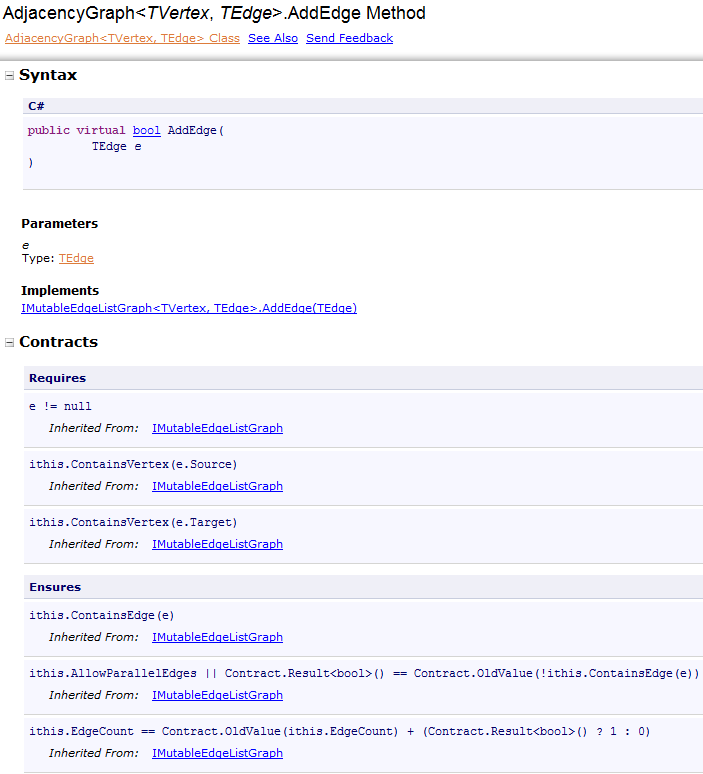
\includegraphics[width=1.05\columnwidth]{docexample.png}
\end{center}
\caption{Generated Documentation with Contracts}
\label{fig:doc}
\end{figure}
\end{center}


\subsection{Documentation Generation}
\noindent
Contracts enable programmers to document design decisions for future
reference. These design decision may be about methods internal to a
component, or public APIs. Contracts on component internal methods
come in handy during code maintenance, which is often done by
programmers other than the original author. For public APIs, contracts
provide programmers with unambigous descriptions of the API they are
trying to use, complementing any natural language documentation.

Thus, generating good documentation from the embedded contracts is a
key scenario when using an embedded contract language. Most
programming languages and platforms come with tools that generate API
documentation (web pages and help files) from idiomatic comments in
the code, such as JavaDocs and .NET XML doc comments.

We have prototyped an extension this documentation generation approach
for .NET where we augment the XML documentation file of .NET
assemblies with new elements for contracts based on the corresponding
contract reference component and the original source text of
preconditions, postconditions, and object invariants.

The resulting XML file can then be rendered into documentation with an
existing tool such as Sandcastle
(\url{http://www.codeplex.com/Sandcastle}), which only requires
patching a few XSL transforms.  An example of the generated
documentation is presented in Figure~\ref{fig:doc}.

As is visible in the example, a key feature of the generated
documentation is that it includes inherited contracts on derived
methods, thereby making it easier to discover contracts than if they
were another hyperlink away.

\subsection{Static Contract Checking}
\noindent
Various approaches can be used to attempt to validate contracts
statically. ESC/Java and Spec\# translate a method and its contracts
into a logic verification condition that is then given to a theorem
prover which either discharges it or produces a
counterexample. Alternatively, special purpose static checkers can be
written for subsets of specifications, e.g., those having to do with
nullness of pointers.

Yet another approach is to use abstract interpretation to compute
program invariants and then attempt to use these invariants to
discharge the proof-obligations introduced by contracts. Abstract
interpretation enables more automation than verification condition
approaches due to its ability to infer loop-invariants and
post-conditions. It also enables fine-tuning performance/precision
trade-offs~\cite{LogozzoMaf08}.

Whatever the mechanism used to prove contracts, all contracts can be
viewed as \code{assert} or \code{assume} statements in the code to be
analyzed. E.g., a precondition at a call-site turns into an assertion,
as the precondition needs to be discharged there. The same
precondition at the beginning of the method declaring or inheriting it
turns into an assumption, a condition the rest of the method can
assume and does not need to be proven. Similarly, postconditions on exit of a
method must be treated as asserts, but on return from a method are treated as
assumes. This rely-guarantee view of contracts enables modular static
checking, where each method can be analyzed in isolation (if
desired). Of course, checkers are free to inline methods, or determine
stronger contracts than the declared ones, thereby performing more
global analyses.

Our approach advocates performing the static contract checking on the
target language of the compiler, as this is how we associate semantics
with contract conditions. Note that contract conditions and ordinary
code therefore use the same language and the analysis is thus simpler
than if these were two distinct code representations. Furthermore,
analyzing the target language of a compiler is often simpler, as it is
usually smaller than a source language in terms of complexity and
number of distinct language elements~\cite{LogozzoMaf08-2}.

The presence of CRC's again provides the necessary access to contracts
of components being called from a component $A$ under analysis. To
analyze $A$, we thus need $A.Contracts$, as well as $B.Contracts$ for
all components $B$ referenced from $A$.


\section{Conclusion}
\noindent
This paper argues for embedding a contract language inside
an existing, standard, production quality language instead of
inventing custom contract annotations or comment
conventions. Embedding contracts means expressing specifications
 as expressions in the existing programming language and
making them machine discoverable through the use of marker methods
such as \code{Contract.Requires}. 

Advantages of embedding a contract language are that programmers need
not learn a new specification language, and existing tools such
as compilers and IDEs can be used without modification, making it
easier for developers to adopt contract-based
programming. Furthermore, the semantics of contract conditions is the
same as the semantics of the existing program expressions. The target
language provides an automatic persisted format for contracts.

Since contract expressions are compiled by the existing compiler, the
typical problem of having the specifications and the code drift apart
due to edits, refactoring, etc., is avoided.


\bibliographystyle{plain}
%\bibliography{cc}
\begin{thebibliography}{10}

\bibitem{Ball04slamand}
Thomas Ball, Byron Cook, Vladimir Levin, and Sriram~K. Rajamani.
\newblock {SLAM} and static driver verifier: Technology transfer of formal
  methods inside {Microsoft}.
\newblock In {\em Integrated Formal Methods}, pages 1--20. Springer, 2004.

\bibitem{SpecSharp}
Mike Barnett, K.~Rustan~M. Leino, and Wolfram Schulte.
\newblock The {Spec\#} programming system: An overview.
\newblock In {\em CASSIS}, volume 3362 of {\em LNCS}. Springer, 2004.

\bibitem{adaspark}
Bernard Carr\'{e} and Jonathan Garnsworthy.
\newblock {SPARK}---an annotated {Ada} subset for safety-critical programming.
\newblock In {\em TRI-Ada '90: Proceedings of the conference on TRI-ADA '90},
  pages 392--402. ACM, 1990.

\bibitem{vcc}
Markus Dahlweid, Michal Moskal, Thomas Santen, Stephan Tobies, and Wolfram
  Schulte.
\newblock {VCC}: Contract-based modular verification of concurrent {C}.
\newblock In {\em 31st International Conference on Software Engineering, ICSE
  2009, May 16-24, 2009, Vancouver, Canada, Companion Volume}, pages 429--430.
  IEEE, 2009.

\bibitem{OpalDas06}
Manuvir Das.
\newblock Formal specifications on industrial-strength code-from myth to
  reality.
\newblock In {\em Computer Aided Verification, 18th International Conference,
  CAV 2006}, page~1, 2006.

\bibitem{Deline04typestatesfor}
Robert Deline and Manuel Fahndrich.
\newblock Typestates for objects.
\newblock In {\em Proceedings of the 18th European Conference on
  Object-Oriented Programming}, pages 465--490. Springer, 2004.

\bibitem{nonnull}
Manuel F\"{a}hndrich and K.~Rustan~M. Leino.
\newblock Declaring and checking non-null types in an object-oriented language.
\newblock In {\em OOPSLA '03: Proceedings of the 18th annual ACM SIGPLAN
  conference on Object-oriented programing, systems, languages, and
  applications}, pages 302--312. ACM, 2003.

\bibitem{DBLP:conf/popl/Godefroid07}
Patrice Godefroid.
\newblock Compositional dynamic test generation.
\newblock In {\em Proceedings of the 34th ACM SIGPLAN-SIGACT symposium on
  Principles of programming languages}, pages 47--54, 2007.

\bibitem{DBLP:conf/kbse/GuptaMS00}
Neelam Gupta, Aditya~P. Mathur, and Mary~Lou Soffa.
\newblock Generating test data for branch coverage.
\newblock In {\em ASE : IEEE International Conference on Automated Software
  Engineering}, pages 219--228, 2000.

\bibitem{DBLP:journals/cacm/King76}
James~C. King.
\newblock Symbolic execution and program testing.
\newblock {\em Communications of the ACM}, 19(7):385--394, 1976.

\pagebreak

\bibitem{DBLP:journals/tse/Korel90}
Bogdan Korel.
\newblock Automated software test data generation.
\newblock {\em IEEE Transactions on Software Engineering}, 16(8):870--879,
  1990.

\bibitem{Leavens-Baker-Ruby06}
Gary~T. Leavens, Albert~L. Baker, and Clyde Ruby.
\newblock Preliminary design of {JML}: A behavioral interface specification
  language for {Java}.
\newblock {\em SIGSOFT}, 31(3):1--38, March 2006.

\bibitem{datagroups}
K.~Rustan~M. Leino.
\newblock Data groups: specifying the modification of extended state.
\newblock In {\em OOPSLA '98: Proceedings of the 13th ACM SIGPLAN conference on
  Object-oriented programming, systems, languages, and applications}, pages
  144--153, 1998.

\bibitem{LogozzoMaf08-2}
F{.} Logozzo and M{.}~A{.} F\"ahndrich.
\newblock On the relative completeness of bytecode analysis versus source code
  analysis.
\newblock In {\em CC'08}, LNCS. Springer-Verlag, March 2008.

\bibitem{LogozzoMaf08}
F{.} Logozzo and M{.}~A{.} F\"ahndrich.
\newblock Pentagons: A weakly relational abstract domain for the efficient
  validation of array accesses.
\newblock In {\em ACM SAC'08 - OOPS}. ACM Press, March 2008.

\bibitem{eiffel}
B{.} Meyer.
\newblock {\em Eiffel: {T}he {L}anguage}.
\newblock Prentice {H}all, 1992.

\bibitem{pluggable}
Matthew~M. Papi, Mahmood Ali, Telmo~Luis Correa, Jr., Jeff~H. Perkins, and
  Michael~D. Ernst.
\newblock Practical pluggable types for {Java}.
\newblock In {\em ISSTA '08: Proceedings of the 2008 international symposium on
  Software testing and analysis}, pages 201--212. ACM, 2008.

\bibitem{DBLP:conf/tap/TillmannH08}
Nikolai Tillmann and Jonathan de~Halleux.
\newblock Pex-white box test generation for {.NET}.
\newblock In {\em TAP: Tests and Proofs Second International Conference}, pages
  134--153, 2008.

\bibitem{DML}
Hongwei Xi and Frank Pfenning.
\newblock Dependent types in practical programming.
\newblock In {\em POPL '99: Proceedings of the 26th ACM SIGPLAN-SIGACT
  symposium on Principles of programming languages}, pages 214--227. ACM, 1999.

\bibitem{Dana}
Dana~N. Xu, Simon L.~Peyton Jones, and Koen Claessen.
\newblock Static contract checking for {Haskell}.
\newblock In {\em Proceedings of the 36th ACM SIGPLAN-SIGACT Symposium on
  Principles of Programming Languages}, pages 41--52. ACM, 2009.

\end{thebibliography}

\end{document}
